\section{Hypergraphs preserve trajectory membership}\label{sec:C15:hypergraph}
HyperSkill represents subtask and skill nodes together with a hyperedge for each experience~\cite{xu2026hyperskill}. The hyperedge retains membership in a common trajectory and carries a task description, distilled lesson, and quality information. This is more specific than a claim that graphs improve memory. The representation keeps an association among several elements that were used together, whereas a flat vector store retrieves each element independently. The benefit must still be evaluated against matched retrieval and evidence budgets.

Let $V=V_u\cup V_s$ be subtask and skill nodes and let $E$ be trajectory hyperedges. A task query $q$ produces a decomposition $P(q)$. One retrieval route matches this decomposition to subtask nodes, then expands to incident hyperedges. A second route matches the task description to trajectory representations. Their union is
\begin{equation}
 E^*=E_{\mathrm{sub}}\cup E_{\mathrm{task}}.
\end{equation}
Candidate skills are members of those retrieved hyperedges. HyperSkill ranks them primarily through retrieved co-occurrence,
\begin{equation}
 \kappa(s)=|\{e\in E^*:s\in e\}|,
\end{equation}
with semantic similarity used for ties. These equations describe the inspected method, not a newly proposed retrieval result.

The representation should not be confused with a magical source of higher-order semantics. A hypergraph can be encoded as a bipartite incidence graph with explicit hyperedge nodes. What matters is retaining trajectory identity and membership, not the use of one graph library. A pairwise projection that discards hyperedge identity can lose which groups co-occurred together, while a representation that preserves the incidence relation can express the same membership. This is a structural deduction that sharpens the comparison axis.

The decomposition route can retrieve procedural analogies that differ lexically at the whole-task level. It can also amplify decomposition errors: if the generated plan misidentifies the task, it steers retrieval toward the wrong experiences. The task-level route provides a complementary signal but does not guarantee correction. A meaningful ablation holds total retrieved evidence fixed and compares task-only, subtask-only, and fused retrieval, with the same downstream model and prompt budget.

Co-occurrence is evidence of repeated use within retrieved experiences, not proof of causal usefulness. A generic skill can appear frequently because it was extracted from many tasks, while a rare exception-handling skill can be decisive. Frequency-based ranking and quality-based maintenance address different concerns. Their interaction should be inspected: pruning a rarely tested item, changing the set of retrieved edges, or merging broad skills can alter the candidate pool before the co-occurrence ranker runs.



Figure~\ref{fig:C15:overview} isolates the mechanism and its stated information boundaries.
\begin{figure}[!htbp]
\centering
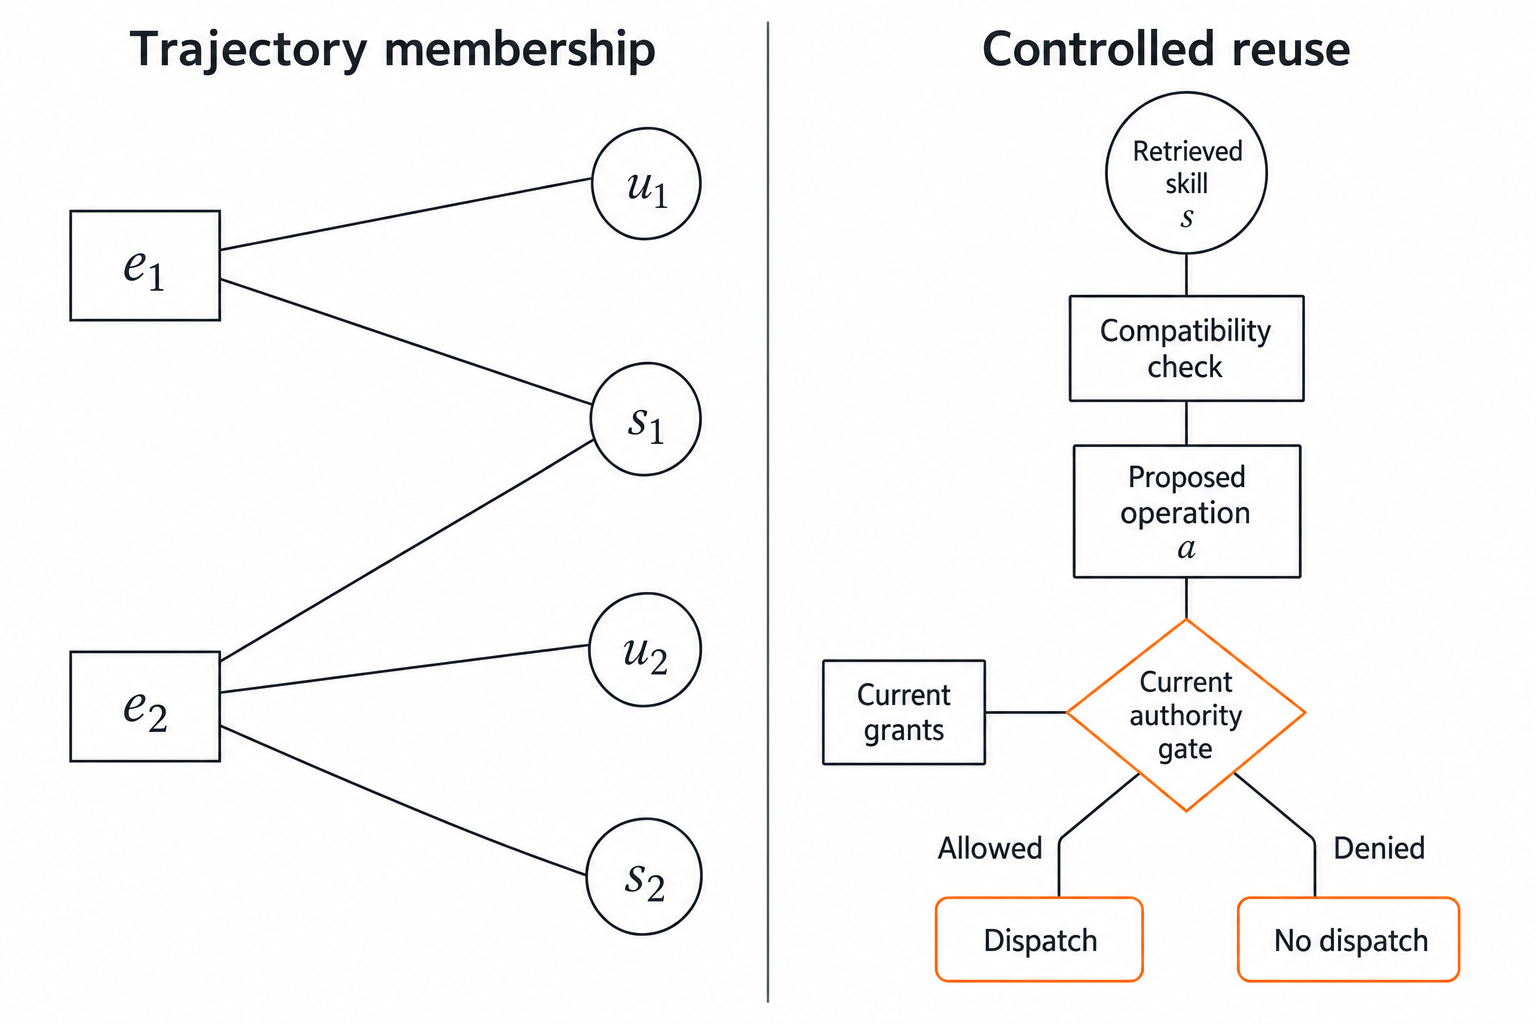
\includegraphics[width=\linewidth]{book/figures/assets/F15review.png}
\caption{An illustrative incidence representation: $e_i$ denote episodes, $u_i$ subtasks, and $s_i$ reusable skills. Undirected lines retain membership, not execution order. A retrieved skill remains a procedural hypothesis; compatibility and the proposed operation's current dispatch authority are separate checks. Neither membership nor compatible metadata proves procedural correctness. Maintenance uses additional evidence outside this schematic. Right-hand connectors show dependencies among checks and labelled conditional outcomes.}
\label{fig:C15:overview}
\end{figure}
